\section{Prac 4A - FPGA Introduction (Archived)}
\label{sec:Prac4}
\subsection{Introduction}
For this practical, it is important to complete the tutorial first to become acquainted with the tools required to complete the practical. It is recommended that you work in groups of three, and that all three members work through the tutorial individually.

It is also imperative that you read through the \href{http://wiki.ee.uct.ac.za/Main_Page}{wiki.ee}. Operation of Vivado can be intimidating at first use. The Wiki has been carefully written to include all you need for the practicals, see the page \href{http://wiki.ee.uct.ac.za/Xilinx_Vivado}{here}. 

\subsection{Tutorial}
The tutorial is not for marks but it is suggested you complete it, as it will give you the basics of Vivado, and allow you to upload a simple program to the FPGA. In the tutorial (as in wiki.ee) we use the Digilent Nexys A7 as an example board, but the process should be the same for the Nexys 4 DDR and Nexys 4. The only thing that will change between the three is the board you select when creating the project, and the constraints file you use. Note the constraints file does determine naming of some of the I/O, so double check that.

Most of the details on how to complete these steps are on the wiki under \href{http://wiki.ee.uct.ac.za/Xilinx_Vivado}.

\begin{enumerate}
    \item Install Vivado
    \item Install boards\\
    The only boards you might work with in this course are the Nexys 4, Nexys 4 DDR, and the Nexys A7. So you only need to worry about installing those.
    \item Download and save the constraint files. That, or copy the simple example given on the wiki if you're using the A7.
    \item Create a new project. 
    \begin{itemize}
        \item You can call it ``Tutorial".
        \item Set it as an RTL project and select ``Do not add sources at this time". For the prac later, you can add the given source files here.
        \item Select your board appropriately.
    \end{itemize}
    \item Add constraint source
    \begin{itemize}
        \item Right click on constraints, select "Add sources". In the dialog box, make sure ``Add or create constraints" is selected. Hit next.
        \item Select ``Create file" if you are copy pasting the constraints in, or ``add files" if you have the constraints file downloaded locally. Press ``Finish".
        \item If you were intending on copy-pasting constraints in, do so now. Ensure your constraints are correct for the board, and have the clock, two switches and two LEDs enabled.
        \item Right click on the constraints file, and select "Set as Target Constraint File"
    \end{itemize}
    \item Add the Verilog source
    \begin{itemize}
        \item Right click on ``Design Sources'', select ``Add sources''. In the dialog box, make sure ``add or create design sources'' is selected. Hit next.
        \item Select ``Create file". Call it the same name as your project (good practice for the top level module). Press ``Finish''.
        \item A dialog will open, with ports. You can just press ``okay", as we'll define ports in the Verilog code.
        \item Right click on the Verilog file, and select ``Set as Top" (if it is not already set as top - indicated by being in bold).
        \item In it, paste code to, each clock cycle, write switch[0] to LED[0] and the inverse of switch[1] to LED[1]. Example code can be found on the wiki.
    \end{itemize}
    \item Select ``Run Synthesis"
    \item Select ``Run Implementation"
    \item Select ``Generate Bitstream"
    \item Upload your bitstream to your target board (speak to a tutor to get a board)
    \begin{enumerate}
        \item Plug in the board
        \item Select ``Open Hardware Manager"
        \item Select ``Open Target" and then "Auto Connect"
        \item Vivado should find the board. Select ``Program Device" and select the board you've plugged in (The A7 shows as ``xc7a100t\_0". Press the "Program" button.
    \end{enumerate}
    \item Hooray! You've created your first FPGA circuit. Toggle the switches to see if it operates as expected. Now let's move on to the fun stuff.
\end{enumerate}

\subsection{Practical}
\subsubsection{Introduction}
In this practical, you will create a digital clock on an FPGA. There is no report for the practical, but you will need to submit screenshots of your testbenches and demonstrate your implementation to a tutor.

Source files are available on the EEE4120F OCW GitHub: \href{https://github.com/UCT-EE-OCW/EEE4120F-Pracs}{https://github.com/UCT-EE-OCW/EEE4120F-Pracs}.


\subsubsection{Given Modules}
\begin{enumerate}
    \item TLM\\
    The top level module, called "Clock.v" in the source files on GitHub, contains the primary logic for your wall clock and allows you to implement I/O and other modules
    \item Delay\_Reset\\
     It's also useful as many components require a set up time. So by using a delayed reset signal, we can cater for reset times of peripherals.
    \item Seven-Segment Driver\\
    This module takes 4 BCD values and displays them on the seven segment display.
    \item Decoder\\
    Used by the Seven-Segment Driver to decode decimal to the appropriate cathode pins.
    \item Debounce\\
    A debounce module you'll need to implement in order to debounce button presses.
    \item PWM\\
    A module you'll need to implement in order to give the seven segment displays changing brightness. This can be tricky, it's suggested you leave it for last.
\end{enumerate}

\subsubsection{Requirements}
The following outcomes are required to pass the demonstration:
\begin{enumerate}
    \item Implement a simple state-machine to display the real time (hours and minutes) on the 7-segments display. You can start your clock at 00:00 upon reset. Make your clock faster in order to test that the time overflows correctly. Use a 24-hour time format. 
    
    The easiest way to do this is with deeply nested if statements. Run a counter that overflows every second and increment the seconds counter on every overflow. Every time this seconds counter equals 59 (i.e. it will overflow on this clock-cycle), increment a minutes units counter. Every time this minutes units counter is about to overflow, increment a minutes tens counter, etc. 
    
    Only use non-blocking assignments ($<=$). Blocking assignments (=) inside clocked structures are much more difficult to debug. Remember that the entire always block is evaluated at once: the statements are not evaluated sequentially.
    \item Display the seconds on the LEDs, in binary format. This is done with a simple assignment outside the always block.
    \item Use one of the buttons, properly debounced, to set the minutes. It must increment time by one minute every time it is pressed. Make sure that your time overflows correctly. You do not need to increment the hours when changing the minutes. 
    
    It is recommended to write a Debounce module for this. On every clock cycle of the system clock (the fast one), check the state of the button. If it is not the same as the current module output, change the output and start a dead time counter. While this counter is counting, do not change the output of the module, no matter what the input is doing. Use a deadtime of between 20 ms and 40 ms. To prevent unstable states, register the button before use. 
    
    In the clock state machine, you can use a register to store the button's `previous' state. If the current state is high, and the previous state is low, the button signal went through a rising-edge. Do not use always @(posedge Button) – keep everything in the same clock domain.
    \item Use another one of the buttons, properly debounced, to set the hours. It must increment time by one hour every time it is pressed. Make sure that your time overflows correctly.
    \item Use the slide-switches to represent a binary “brightness” word. Make use of pulse-width modulation (PWM) to dim the brightness of the LED display. 
    
    Ensure that the phasing between the driver signals and the PWM signals is correct. The easiest way to do this is to select a PWM frequency such that the PWM signal goes through exactly one period between driver signal state changes. You can implement this within the SS Driver module.
\end{enumerate}

\subsection{Mark Allocations}
% Please add the following required packages to your document preamble:
% \usepackage{graphicx}
% \usepackage[normalem]{ulem}
% \useunder{\uline}{\ul}{}
\begin{table}[H]
\centering
\caption{Prac 4 mark allocation}
\label{tbl:Prac4-Marks}
\resizebox{\textwidth}{!}{%
\begin{tabular}{|l|l|l|}
\hline
{\ul \textbf{}} & {\ul \textbf{}} & \textbf{Marks} \\ \hline
\textbf{Testbench} &  & 12 \\ \hline
 & Minute seconds reaching 60 and increasing minutes &  \\ \hline
 & Minutes reaching 59 and increasing hours &  \\ \hline
 & Time reaching 23:59 and wrapping back to 00:00 &  \\ \hline
 & (3 each +3 for neatness) &  \\ \hline
\textbf{Demo} &  &  \\ \hline
 & \begin{tabular}[c]{@{}l@{}}Time flows correctly (minutes overflow to an increase in hours, \\ and 23:59 flows to 00:00)\\ {[}6, subtracting 2 for each missed objective{]}\end{tabular} & 6 \\ \hline
 & \begin{tabular}[c]{@{}l@{}} Time can be scaled through a variable (i.e. the count to \\ increase seconds isn't fixed)\end{tabular} & 2 \\ \hline
 & Minute button increases minutes and doesn't increase hours & 2 \\ \hline
 & Hour button increases hours & 1 \\ \hline
 & Debounce module implemented & 2 \\ \hline
 & PWM module & 5 \\ \hline
 & \textbf{TOTAL} & 30 \\ \hline
\end{tabular}%
}
\end{table}

\textbf{For the 5 marks on PWM}: 1 mark for attempted, 2 marks for reading switches and adjusting, 3 marks for "flashing" implementation, 4 marks for some mix between flashing and decent PWM, 5 marks for correctly implemented.





\section{Prac 4B - Vivado IP and Resource Usage (archived)}
\label{sec:Prac4}
FPGAs are often used in DSP applications due to their highly parallelizable nature and ability to process data at high speeds. Usually FPGAs are used to sample signals and process them, but in this application we're going to generate waveforms and output them to a speaker!

If you aren't all that well acquainted with the physics of music, \href{https://www.youtube.com/watch?v=i_0DXxNeaQ0}{this video by Vihart}\footnote{https://youtu.be/i\_0DXxNeaQ0} is a really great introduction! She speaks quite quickly, so you may need to watch it twice.

These videos don't have much to do with this prac, but are fun to learn about. If you'd like to learn more about modular synthesis (which is super cool!) check out \href{https://www.youtube.com/watch?v=cWslSTTkiFU}{this video by Andrew Huang}!\footnote{https://youtu.be/cWslSTTkiFU} LookMumNoComputer also does a great bunch of custom modular synthesis projects - just check out his \href{https://youtu.be/GYLBjScgb7o}{Furby Organ}!\footnote{https://youtu.be/GYLBjScgb7o} He also has guides on how to \href{https://www.youtube.com/watch?v=4Kz8YopLTCQ&list=PLluPQLh1xzlIzqgTBwTo_a5k_O63JxwjQ}{build your own modular synth}.\footnote{https://youtu.be/4Kz8YopLTCQ}

We'll be implementing a sine wave - which you don't really hear much in music. But as \href{https://www.youtube.com/watch?v=xLtTMkMr2Wg}{Composerly shows us}\footnote{https://www.youtube.com/watch?v=xLtTMkMr2Wg}, you can create some greate tunes with nothing but sine waves and enough processing.

\subsection{Tutorial}
The tutorial starts with guidance on getting familiar with the Xilinx Vivado IP facilities, which leads in to the requirements for the prac. 

\subsubsection{Resource usage}
Please read the \href{http://wiki.ee.uct.ac.za/Xilinx_Vivado#Implement}{Implement section} in the Xilinx Vivado page on the UCT EE Wiki.

\subsubsection{Vivado IP}
For general information on the Vivado IP, please read the "Xilinx Vivado IP" section of the \href{http://wiki.ee.uct.ac.za/Xilinx_Vivado#Xilinx_Vivado_IP}{Xilinx Vivado wiki page}.

Of course, when using an IP core, you need to have some knowledge of the technology. You should know how to use the IP cores - and, since you are university students and not necessarily going to just be users - you should also have some sense of what is happening behind the scenes. \footnote{You'll get a better sense of the theory behind these concepts from the lectures building on the basics of the PLDs and FPGAs covered in ES1 and ES2.} In the tutorial, you will be guided through the relevant settings and what they mean, but when using other IP, you should do your research as to what you're adjusting.



Once you've created your project for your board, you can do the following to instantiate memory to hold the lookup table. You can repeat this process for different tables or waves (for example sawtooth, triangle, or perhaps another periodic waveform - maybe the waveform for a specific instrument).
\begin{enumerate}
    \item Select ``IP Catalogue" on the left hand side of the IDE
    \item Search ``BRAM".
    \item Under ``RAMs \& ROMs \& BRAM", select the "Block Memory Generator"
    \item Select ``Port A Settings"
    \item Note the write and read width. These relate to the bitwidth of the data in the memory. Change this to 11 for both read and write. We use 11 because the audio module expects a signal 11 bits big.
    \item The write and read depth relate to how many samples can be stored. Change this to 256, as out example sine table has 256 samples, and this we need 256 addresses.
    \item Select ``Other Options"
    \item Select ``Load Init File"
    \item Browse to the Prac 4 sources, and load LUT\_sinefull.coe
    \item Click ``Ok" at the bottom of the dialog
    \item Click ``Generate" on the next dialog. Press "Ok" when the information dialog shows up.
    \item In sources view, there will be a template available to instantiate the IP.
    \item Congrats! You've added a 11-bit 256 sample Block RAM IP!
\end{enumerate}

It would be a good idea to set up a test bench to ensure you're reading the correct values from the BRAM as you expect. Here's some hints which might make setting up the test bench easier:
\begin{itemize}
    \item You don't need to do any writing to the BRAM (write enable can be left low)
    \item You can leave the read enable signal high
    \item You can just increase the address by 1 each time - it will auto wrap around to 0
\end{itemize}

\subsection{Practical}
We're going to start by making a simple waveform generator to output middle C at f=261.625565Hz (or as close as you can get to it!). Then we're going to try free up some resources in our first implementation. From there, we're going to create an arpeggiator. If you're familiar with synthwave - it's usually an arpeggiator (or \textit{arp}) that creates the repetitive notes in the background.

\subsubsection{Provided files}
You are provided with:
\begin{enumerate}
    \item top.v\\
    The top level module for the project. A template to get you started.
    \item pwm.v\\
    A PWM module to convert the BRAM samples to a PWM signal for the audio jack.
    \item LUT\_sinefull.coe\\
    A full sinewave table, 11 bits wide with 256 samples
\end{enumerate}

\subsubsection{Creating a waveform generator}
In this section you need to create a simple output waveform generator at as close to 261.625565Hz as you can. The hardware operates at 100MHz, so 100Mhz/(261.62556Hz*256) gives us 382225.643736. But! We have 256 samples in our look up table. So we need to operate 256 times faster to complete one wave in the expected time. 382225.643736 divided by 256 is about 1493. So count to that value to produce a tone around middle C.

\begin{enumerate}
    \item Start by creating a new project, and adding the full sine wave table to BRAM as per the tutorial above. A reminder to use the correct board settings when creating a new project and calling it fullsine.
    \item Create a new test bench, showing loading a sample from the BRAM
    \item Record resource usage for the full sine table (we're looking for total power, LUT, FF, BRAM)
    \item Output this wave to the audio port, and record video of it playing. To do so, you need to tie in the AUD\_SD and AUD\_PWM signals from your constraints file. AUD\_SD can be written high (as an enable). AUD\_PWM needs to be a PWM signal. To generate this, pass the data from the BRAM to an instantiation of pwm.v, and pass the output of that PWM module to AUD\_PWM.
\end{enumerate}
\textbf{Create a new project called quartersine} and implement a quarter sine wave table. Record resource usage for this project too, as you will need to compare the implementations later. This resource will be helpful in implementation: \href{https://zipcpu.com/dsp/2017/08/26/quarterwave.html}{https://zipcpu.com/dsp/2017/08/26/quarterwave.html}. Make sure to remember that you only need 256/4 = 64 samples when you instantiate the BRAM on this project.


\subsection{Create a simple major arpeggiator}
A major scale in music sounds ``happy". Minor progressions sound ``sad". We're going to create a major arpeggio generator.
A major arpeggio consists of a base note, a major third and a fifth\footnote{\href{https://www.superprof.com.au/blog/arpeggios-guitar-tips/}{Super simple arpeggio explanation for guitarists}}. As we saw in the Vihart video, this is just maths. If we have a frequency \textit{f}, then the major third is just \textit{f*1.25}, and the fifth is just \textit{f*1.5}. We will finish off the arpeggio by completing the octave, which will be \textit{f*2}.
\begin{figure}[H]
\centering
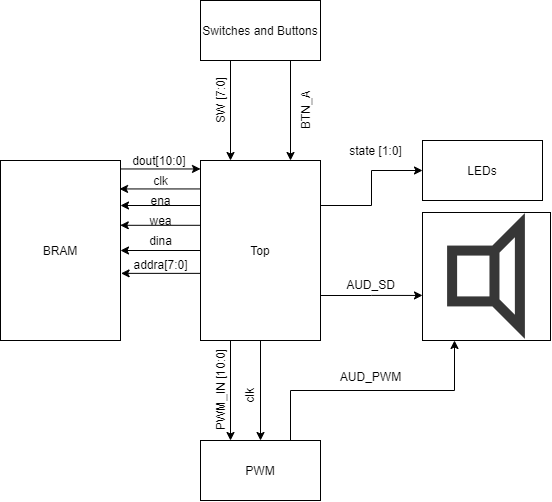
\includegraphics[width=0.6\columnwidth]{Figures/Prac5_BlockDiagram}
\caption{The overview block diagram}
\label{fig:prac4_block}
\end{figure}

So let's think about what we need to do to implement this:
\begin{itemize}
    \item We need a counter to change the note every 500ms
    \item We will need a case statement, which, depending on the note, will change the rate at which we switch through the BRAM address
    \item We will need to read in switches to add to the base note we've chosen (middle C)
    \item We will need a state to hold whether we are sending out an arpeggio, or just out base note.
\end{itemize}

With these items in mind, we know our always block might look something like this. In the code I wrote, I made f\_base the highest frequency (lowest count). The example is very simple, and doesn't cater for switching between f\_base output and arpeggio output. It is just meant to serve as a guide.

\begin{lstlisting}[caption={Example of ``Top" for switching between notes}]
always @(posedge CLK100MHZ) begin   
    PWM <= douta; // tie memory to the PWM out
    
    f_base[8:0] = 746 + SW[7:0]; // get our base frequency
    
    note_switch = note_switch + 1; // keep track of when to change notes
    if (note_switch ==  50000000) begin
        note = note +1;
        note_switch = 0;
    end

    // Output divider to control frequency
    clkdiv <= clkdiv + 1;
    
    case(note) 
        0: begin // base note
            if (clkdiv >= f_base*2) begin
                clkdiv[12:0] <= 0;
                addra <= addra +1;
            end
        end
        1: begin //1.5 times faster
            if (clkdiv >= f_base*3/2) begin
                clkdiv[12:0] <= 0;
                addra <= addra +1;
            end
        end
        2: begin // 1.25 faster
            if (clkdiv >= f_base*5/4) begin
                clkdiv[12:0] <= 0;
                addra <= addra +1;
            end
        end
        3: begin //2 times faster
            if (clkdiv >= f_base) begin
                clkdiv[12:0] <= 0;
                addra <= addra +1;
            end
        end
        default: begin // Don't know what's happening, just output middle C
            if (clkdiv >= 1493) begin 
                clkdiv[12:0] <= 0;
                addra <= addra +1;
            end
        end
    endcase;
    
end
\end{lstlisting}

\subsection{Hand In}
Submit the following as a single PDF:
\begin{enumerate}
    \item Show evidence that the two implementations produce the same results. To do this:
    \begin{itemize}
        \item Show screen captures of the test benches at t=0, t= 1/2 pi and t = pi (we're looking to see the changes in values in the output sine value at these points.) [6 marks]
        \item To further elaborate on the above - we want to see that the value passed to the PWM module on either side of those values of t follow the same progression.
    \end{itemize}
    \item List the resource and power usage of the both implementations [5 marks]
    \item Write a paragraph or two on resource consumption of the FPGA. Talk about resource availability, resources used, effort in terms of implementation  [5 marks]
\end{enumerate}

Submit a video on YouTube showing the arpeggiator working. Make sure to have the volume loud enough. Please describe what you are showing in the video. [10 marks] 
The video should show the following:
\begin{itemize}
    \item In base\_f mode, toggle the switches to show that the frequency changes.
    \item Enable arpeggio mode and show that works by recording the output from a speaker
    \item Change the output frequency while in arpeggiator mode
\end{itemize}